\section{The ``b-tag formula method''}
\label{sec:formula}

In order to maximise sensitivity to potential new physics signatures
in final states with multiple b-quark jets, a method that improves the
statistical power of the simulation, particularly for high btag bins, is
employed. This method is known as the ``formula'' method. The
resulting improvement in the statistical precision of the simulation
propagates through to the transfer factors used in the analysis.

\subsection{Method}
\label{sec:formula-method}

The distribution of the number of bjets (\nb) is estimated from generator-level information
contained in the simulation. The number of reconstruction-level jets
matched to underlying bottom quarks ($\nb^{\rm gen}$), charm quarks
($n_{\rm c}^{\rm gen}$), and light-flavoured partons, i.e. $u,d,s$ quarks and gluons ($n_{\rm
  l}^{\rm gen}$) per event, $N(\nb^{\rm gen},n_{\rm c}^{\rm
  gen},n_{\rm l}^{\rm gen})$, is recorded in bins of (\njet
   , \scalht, \mht). 
 The matching between truth-level partons
and reconstruction-level jets is achieved with a matching algorithm
recommended by the BTV POG~\cite{btagMCTools}.
 The b-tagging efficiency, $\epsilon_{\rm b}$, and mistag probabilities,
$\epsilon_{\rm c}$ and $\epsilon_{\rm l}$, are also determined from simulation
in bins of (\njet,~\scalht,~\mht), with each quantity averaged
over jet $p_{\rm T}$ and $\eta$. Corrections are applied on a
jet-by-jet basis to both $\epsilon_{\rm b}$, $\epsilon_{\rm c}$, and $\epsilon_{\rm l}$
in order to match the corresponding measurements from
data. These corrections, or ``scale factors'', are provided by the BTV POG~\cite{btagMCTools}.

The above information is sufficient to predict the total number of b-tagged jets in the event $n^{\rm tag} \equiv n_{\rm b}^{\rm tag} + n_{\rm c}^{\rm tag} + n_{\rm l}^{\rm tag}$ and thus also
determine the event yield $N(n^{\rm tag})$ from simulation for a given
bin in (\njet,~\scalht,~\mht) with the expression:

\begin{equation}
  \label{equ:btag-formula}
  N(n^{\rm tag}) = \sum_{n_{i}^{\rm gen}} N(n_{\rm b}^{\rm gen},n_{\rm c}^{\rm gen},n_{\rm l}^{\rm gen}) \times (\sum_{n_{i}^{\rm tag}}P_{\rm b}\times P_{\rm c} \times P_{\rm l})
\end{equation}

where $n_{\rm b}^{\rm tag}$, $n_{\rm c}^{\rm tag}$ and $n_{\rm l}^{\rm tag}$ are the number of reconstructed and b-tagged jets 
which are matched to a $b,c$ and $l$ quark respectively and 
$P_{i} = P_{\mathrm{binomial}}(n_{i}^{\rm tag}; n_{i}^{\rm gen}, \epsilon_{i})$ is the usual binomial probability density.

As a simple example, consider a bin with 2 reconstructed jets, in which 
1000 events contain 2 light-jets, i.e. $(n_{\rm b}^{\rm gen} = 0,n_{\rm c}^{\rm gen} = 0,n_{\rm l}^{\rm gen} = 2)$ and 
500 events contain 1 light-jet and 1 b-jet, i.e. $(n_{\rm b}^{\rm gen} = 1,n_{\rm c}^{\rm gen} = 0,n_{\rm l}^{\rm gen} = 1)$. 
In this exercise, we assume a b-tag efficiency $\epsilon_{\rm b} = 0.65$ and a light-tag efficiency $\epsilon_{\rm l} = 0.01$. 
The MC yields for the 3 b-tag multiplicities are then calculated as follows:

\begin{align*}
%% \begin{split}
N(0) &= 1000\times (1-\epsilon_{\rm l})^2 \\
     &+ 500\times (1-\epsilon_{\rm b})\times(1-\epsilon_{\rm l}) = 1153.35 \\
N(1) &= 1000\times (1-\epsilon_{\rm l})\times \epsilon_{\rm l} \times 2 \\
     &+ 500\times (1-\epsilon_{\rm b})\times\epsilon_{\rm l} \\
     &+ 500\times \epsilon_{\rm b} \times (1-\epsilon_{\rm l})\times = 343.3 \\
N(2) &= 1000\times \epsilon_{\rm l}^2 \\
     &+ 500\times \epsilon_{\rm b} \times \epsilon_{\rm l} = 3.35 \\
%% \end{split}
\end{align*}

  
The method exploits the ability to make precise measurements of
$N(n_{\rm b}^{\rm gen},n_{\rm c}^{\rm gen},n_{\rm l}^{\rm gen})$,
$\epsilon$, $f_{\rm c}$, and $f_{\rm l}$ independently of $n_{\rm
  b}$, which means that event yields for a given b-quark jet
multiplicity can be predicted with a higher statistical precision than
obtained directly from simulation. Precise measurements of $f_{\rm c}$
and $f_{\rm l}$ are particularly important for events with $n_{\rm
  b} \geq 3$, which often occur in the SM because of the presence of
mistagged jets in the event. In this case, the largest background is
\ttbar, with two correctly tagged b-quark jets and an additional
mistagged jet originating from a charm quark or light-flavoured
parton.

\subsection{Validation}
\label{sec:formula-validation}

Predictions from the formula method are used to construct transfer 
factors as described in Section~\ref{sec:backgroundmet} and \mht templates 
as described in Section~\ref{sec:syst-on-shape}. 
In order to validate the implementation of the method 
a closure test is performed where the predictions from the formula method 
are compared to the ones from the ``vanilla'' MC, for every 
(\njet,\scalht,\mht) bin. \\
%% As an additional check, the same closure test is performed using the loose b-tag working point. \\ %FIXME: don't have the plots right now
The results in terms of pulls are presented in Fig.~\ref{fig:formula-validation-singlemu} for the \mj control region. 
A good closure is observed which validates the method and its implementation.

The same kind of closure test is carried out at the transfer factor level \ref{sec:backgroundmet}. %FIXME: fix ref 
Additionally, the check is performed for the ``loose'' and ``tight'' working point of the b-tag discriminator, 
beside the ``medium'', which is used in the analysis. \\
The results of this validation is shown in Fig.~\ref{fig:formula-validation-TF}. 
A good closure is observed also in this case. 

\begin{figure}[h!]
  \centering
  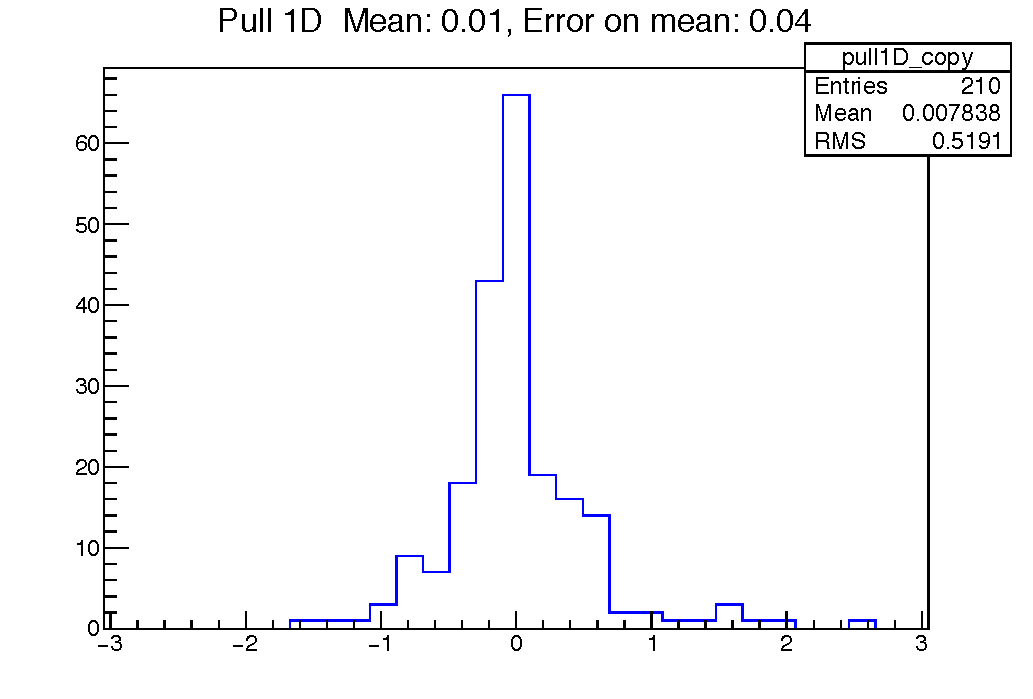
\includegraphics[width=0.45\textwidth]{figures/btagformula/validation/ValidationSingleMu}~
  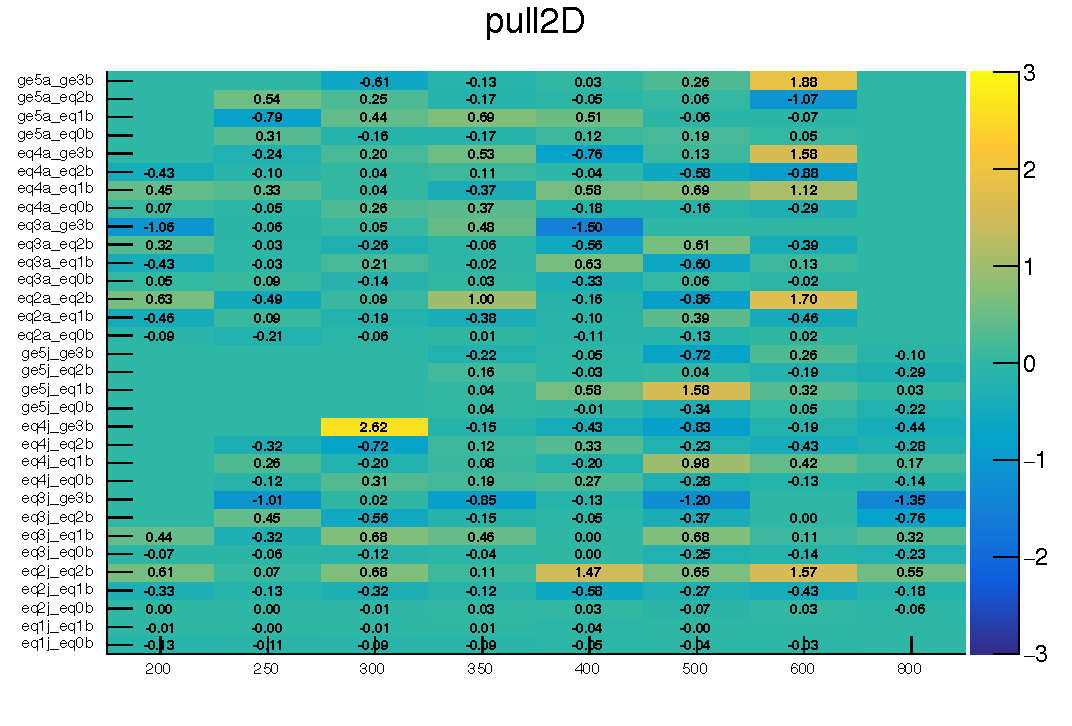
\includegraphics[width=0.45\textwidth]{figures/btagformula/validation/ValidationSingleMu2D} \\
  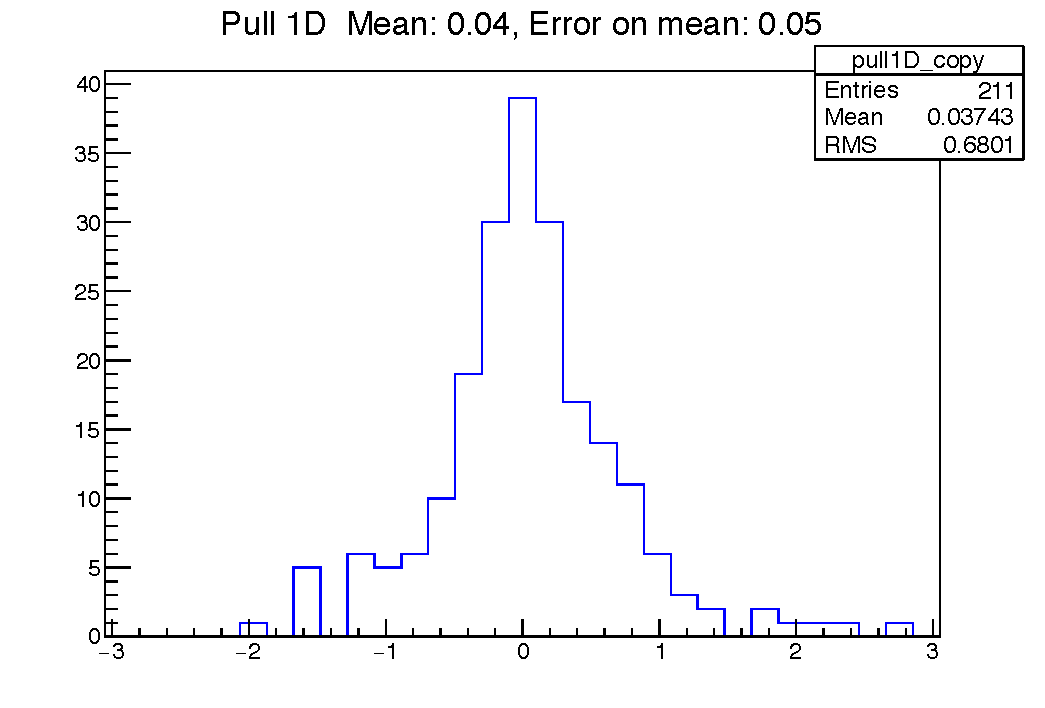
\includegraphics[width=0.45\textwidth]{figures/btagformula/validation/ValidationTTJets}~
  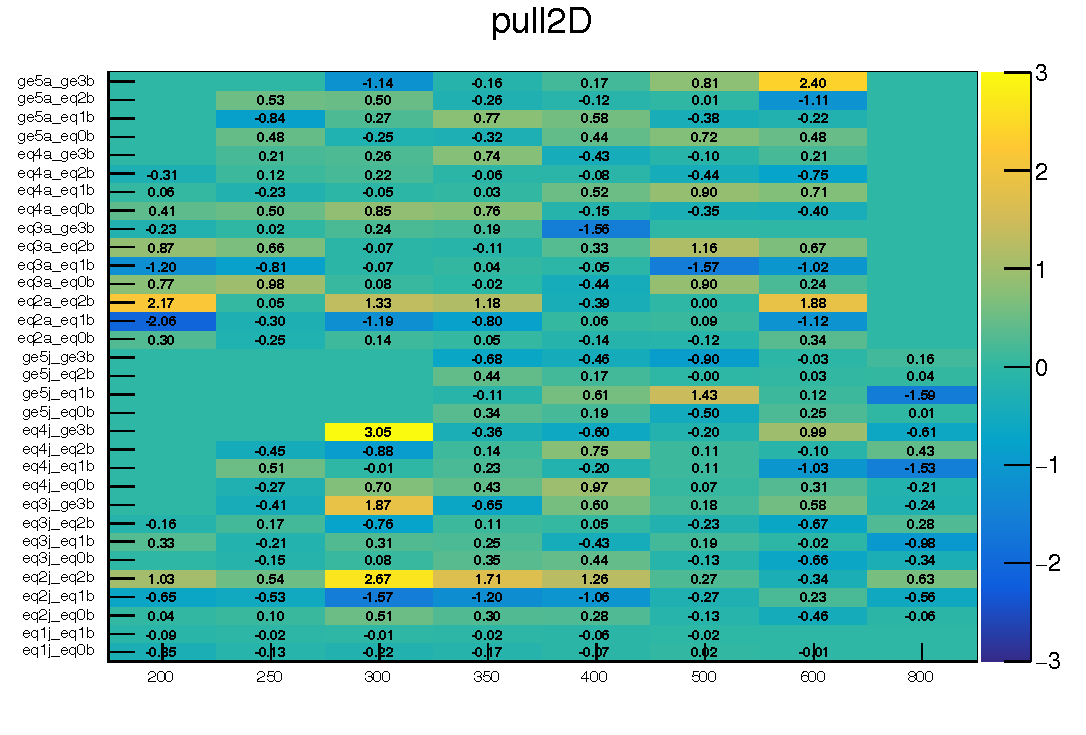
\includegraphics[width=0.45\textwidth]{figures/btagformula/validation/ValidationTTJets2D} \\
  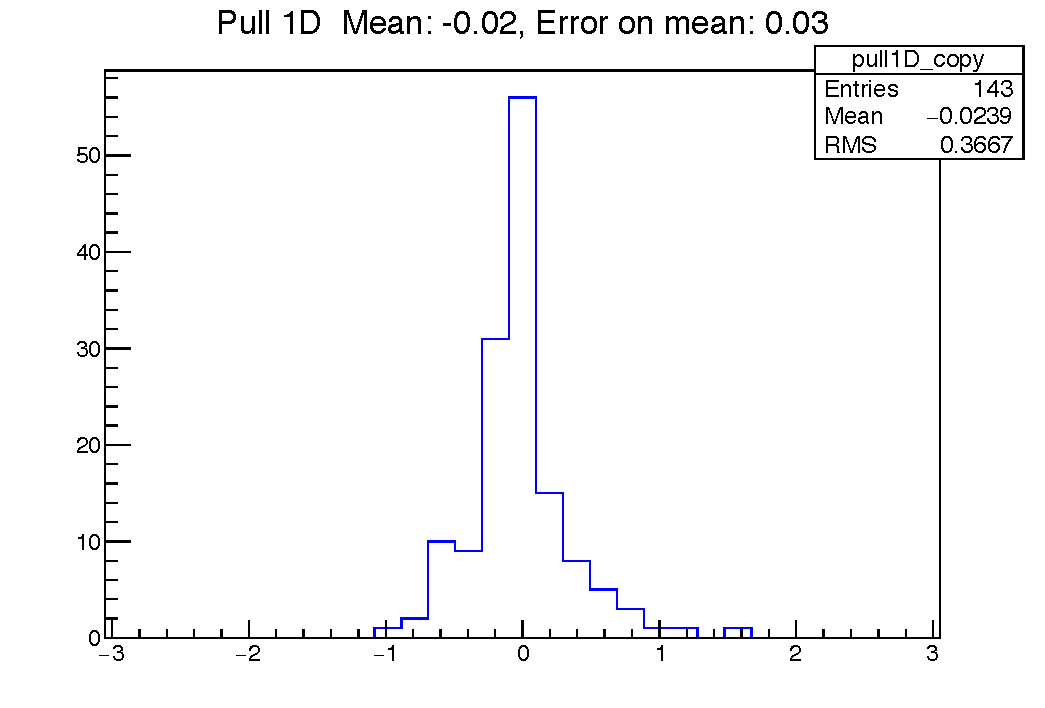
\includegraphics[width=0.45\textwidth]{figures/btagformula/validation/ValidationWJets}~
  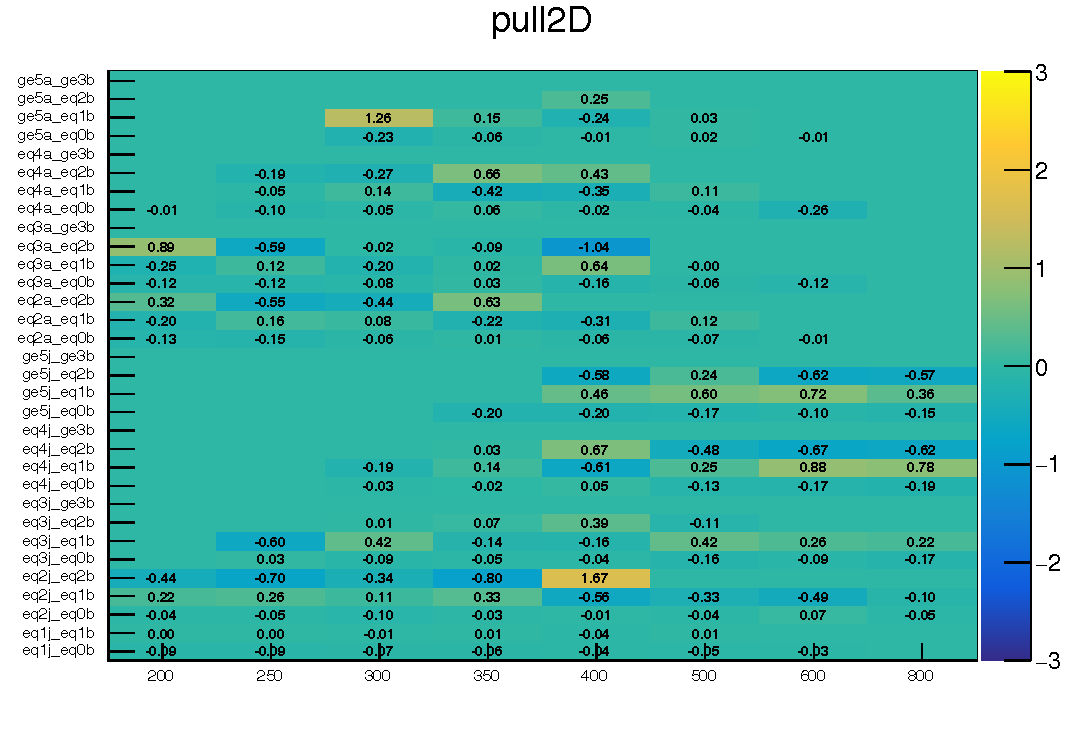
\includegraphics[width=0.45\textwidth]{figures/btagformula/validation/ValidationWJets2D} \\
  \caption{\label{fig:formula-validation-singlemu}
  Inclusive pull distribution (left) and 2D pull distribution as a function of \scalht and (\njet,\nb) bin (right) for
  the total \mj control region yields (top), only the TTJets yields (middle) and only the WJets yields (bottom).
  The pull is defined as the vanilla MC prediction minus the formula method prediction divided by the statistical uncertainty. }
\end{figure}


\begin{figure}[h!]
  \centering
  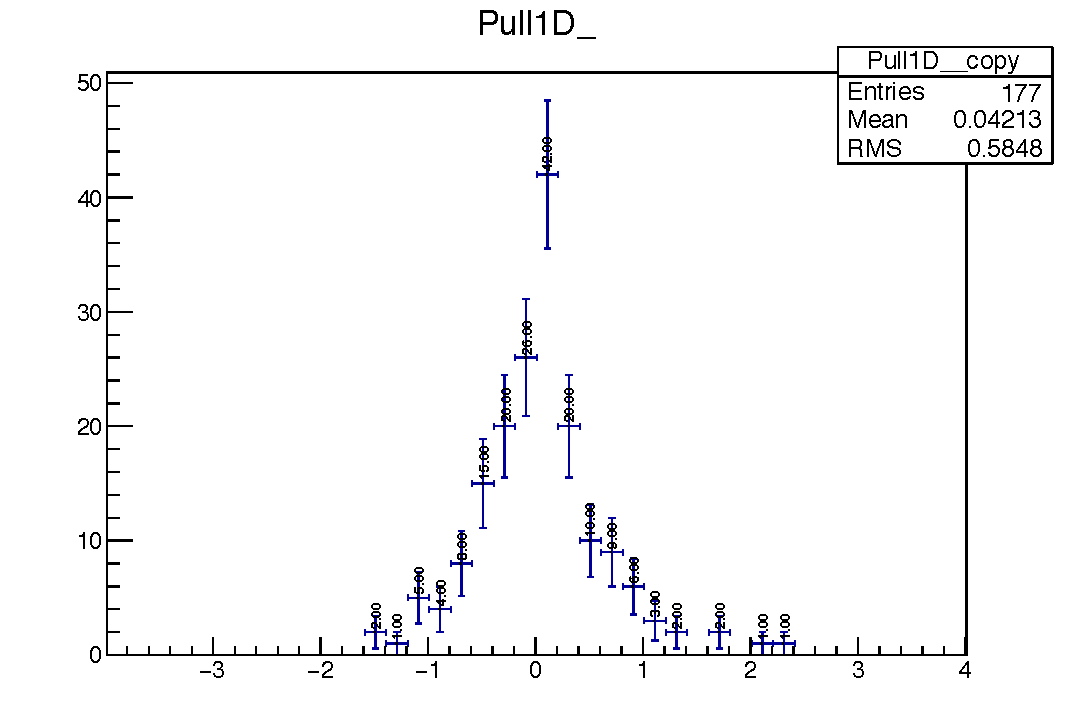
\includegraphics[width=0.45\textwidth]{figures/btagformula/validation/TFValidationSingleMu_loose}~
  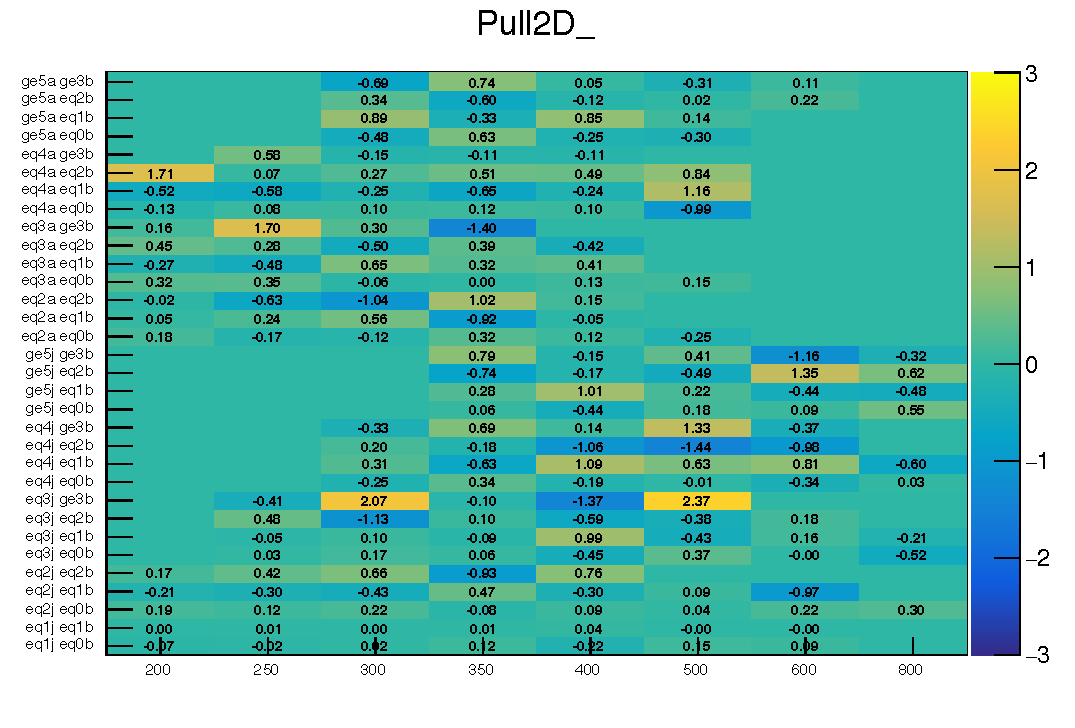
\includegraphics[width=0.45\textwidth]{figures/btagformula/validation/TFValidation2DSingleMu_loose} \\
  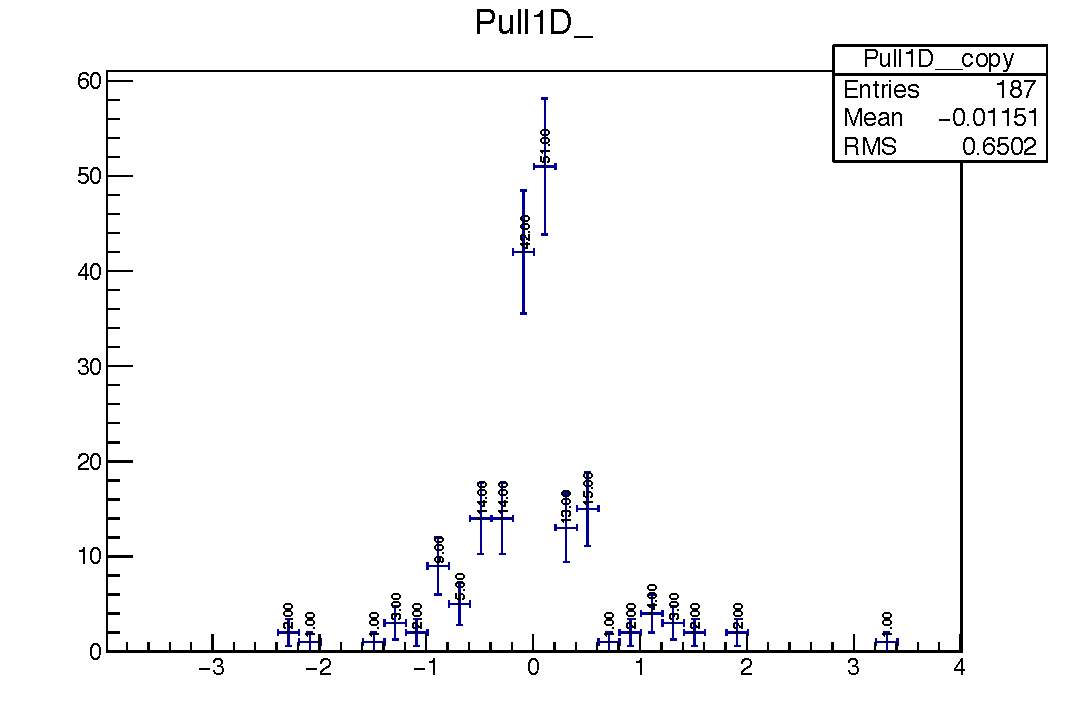
\includegraphics[width=0.45\textwidth]{figures/btagformula/validation/TFValidationSingleMu_medium}~
  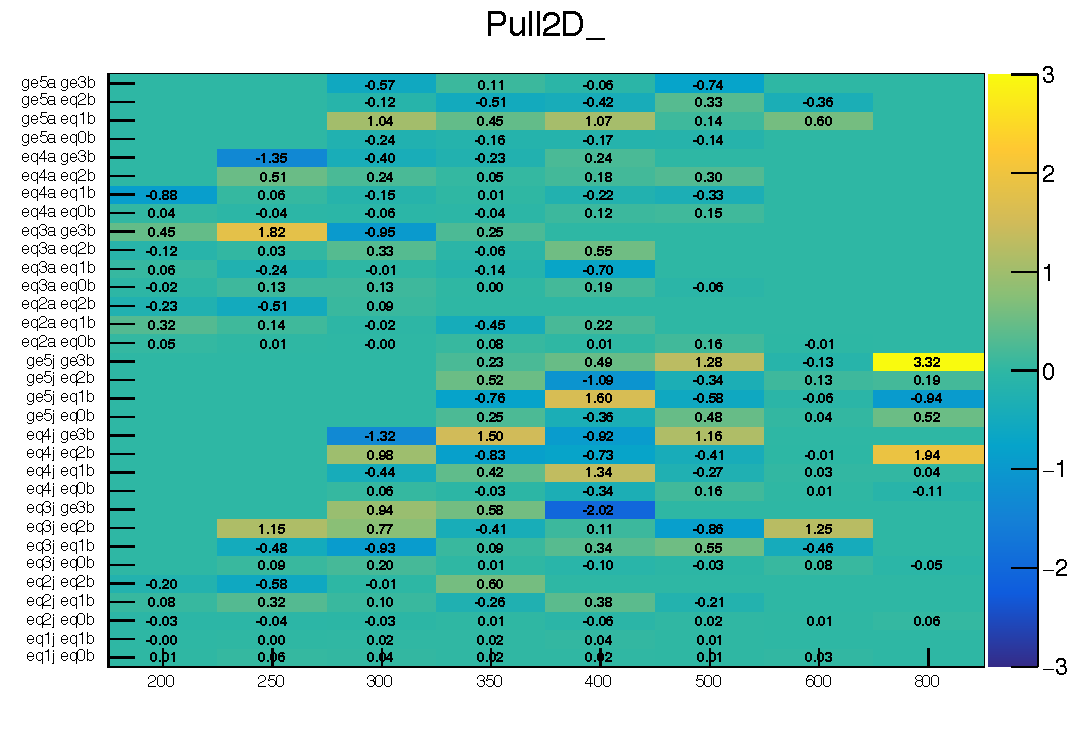
\includegraphics[width=0.45\textwidth]{figures/btagformula/validation/TFValidation2DSingleMu_medium} \\
  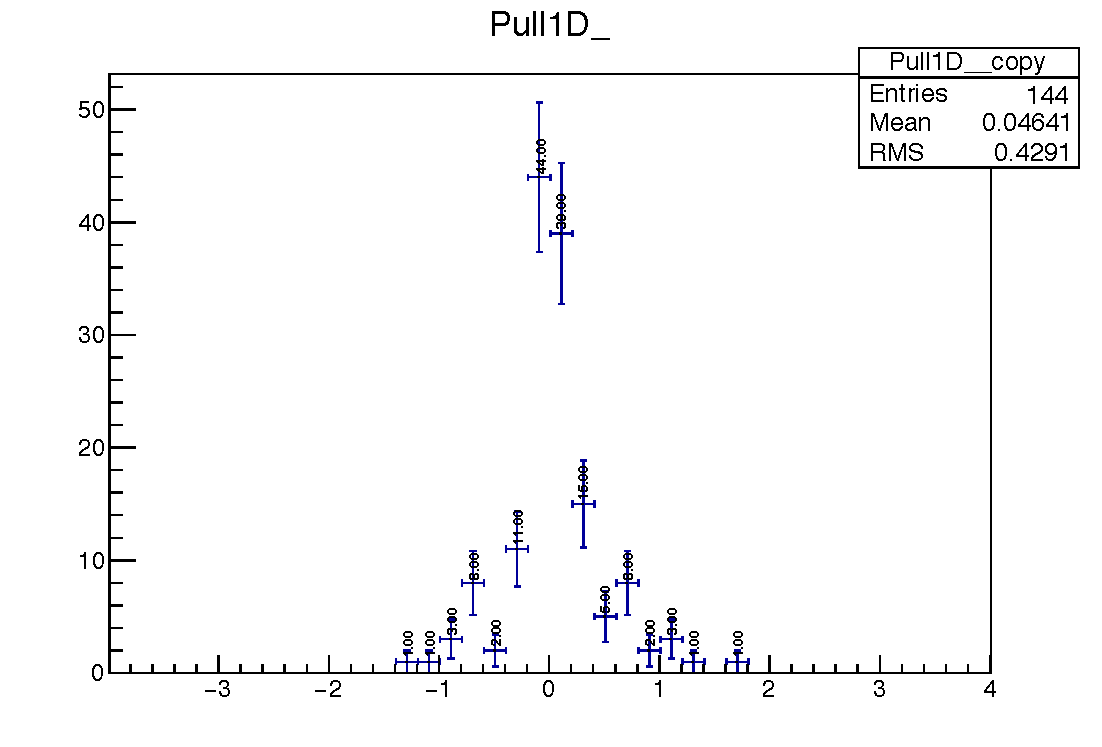
\includegraphics[width=0.45\textwidth]{figures/btagformula/validation/TFValidationSingleMu_tight}~
  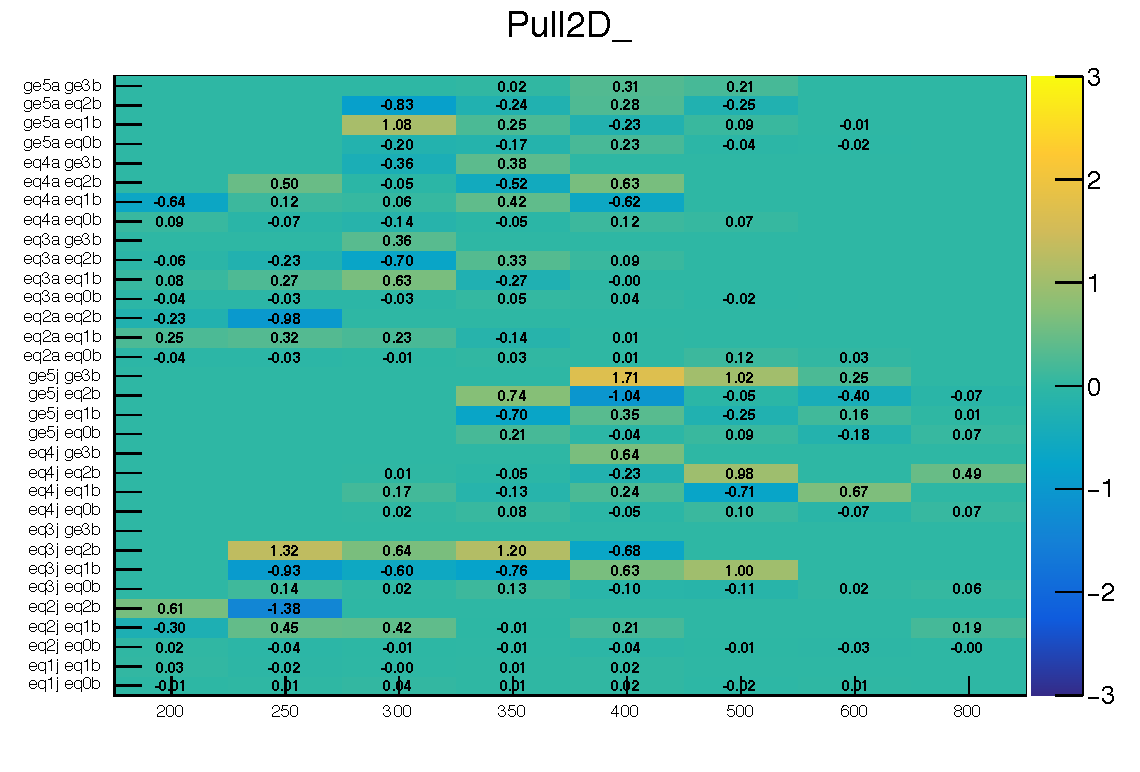
\includegraphics[width=0.45\textwidth]{figures/btagformula/validation/TFValidation2DSingleMu_tight} \\
  \caption{\label{fig:formula-validation-TF}
  Inclusive pull distribution (left) and 2D pull distribution as a function of \scalht and (\njet,\nb) bin (right) for
  the \mj transfer factor (TF) using the loose (top) the medium (middle) and the tight (bottom) working point of the b-tag discriminator. 
  The pull is defined as the vanilla MC TF minus the formula method TF divided by the statistical uncertainty. }
\end{figure}



\subsection{Uncertainties on the predicted MC yields}
\label{sec:formula-uncertainties}
The uncertainties on the MC yields predicted by the b-tag formula method, described in Sec.~\ref{sec:formula-method}, 
are derived by means of a toy procedure. 
A set of 1000 toys is generated randomising the inputs to the method. 
In each toy the $n^{\rm tag}$ distribution is computed after randomising 
the gen-level flavour configuration $N(n_{\rm b}^{\rm gen},n_{\rm c}^{\rm gen},n_{\rm l}^{\rm gen})$ 
from a Poisson statistics and the b-tag efficiencies $\epsilon_{i}$ ($i=\rm b,\rm c,\rm l$) using a Gaussian probability density function. 
The covariance matrix for the $n^{\rm tag}$ bins is then extracted in each (\njet,\scalht,\mht) category and diagonalised. 
From the diagonal terms of this matrix up to 5 un-correlated $n^{\rm tag}$ templates are derived, 
depending on the jet multiplicity in each bin. 
These templates, encoding the uncertainty in the event yield predictions with the b-tag formula method, 
are implemented in the likelihood fit as alternative shapes. 
The uncertainties derived using this procedure effectively replace the bin-by-bin MC statistical uncertainty 
used in the previous iteration of the analysis. 

Fig.~\ref{fig:formula-uncertainties} shows the nominal $n^{\rm tag}$ template and the alternative shapes derived with 
the toy procedure described in this section. 
The statistical uncertainty from the vanilla MC is also shown for comparison. 
From these figures the improvement in the precision of the yield prediction using the formula method can be fully appreciated. 

\begin{figure}[h!]
  \centering
  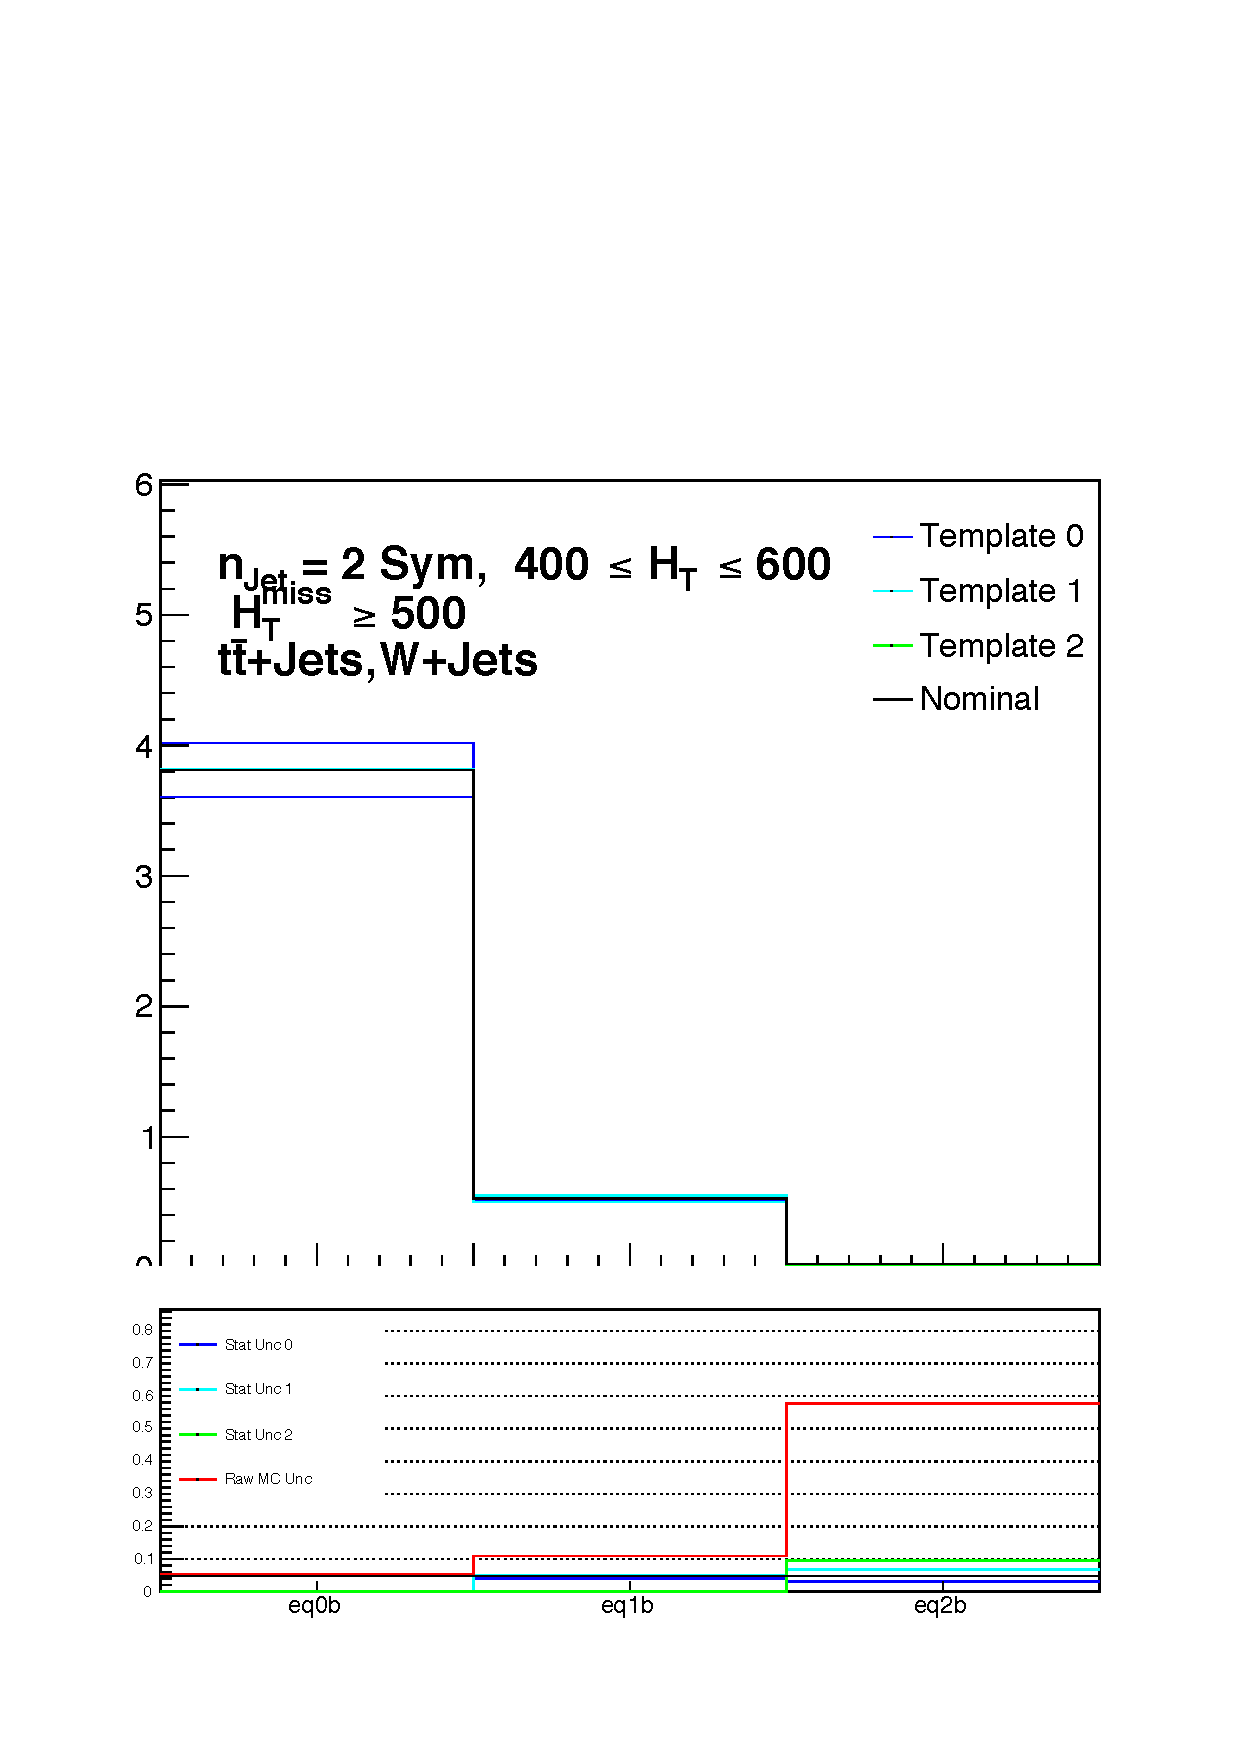
\includegraphics[width=0.45\textwidth]{figures/btagformula/uncertainties/Ttw_eq2j_400600_500Inc}~
  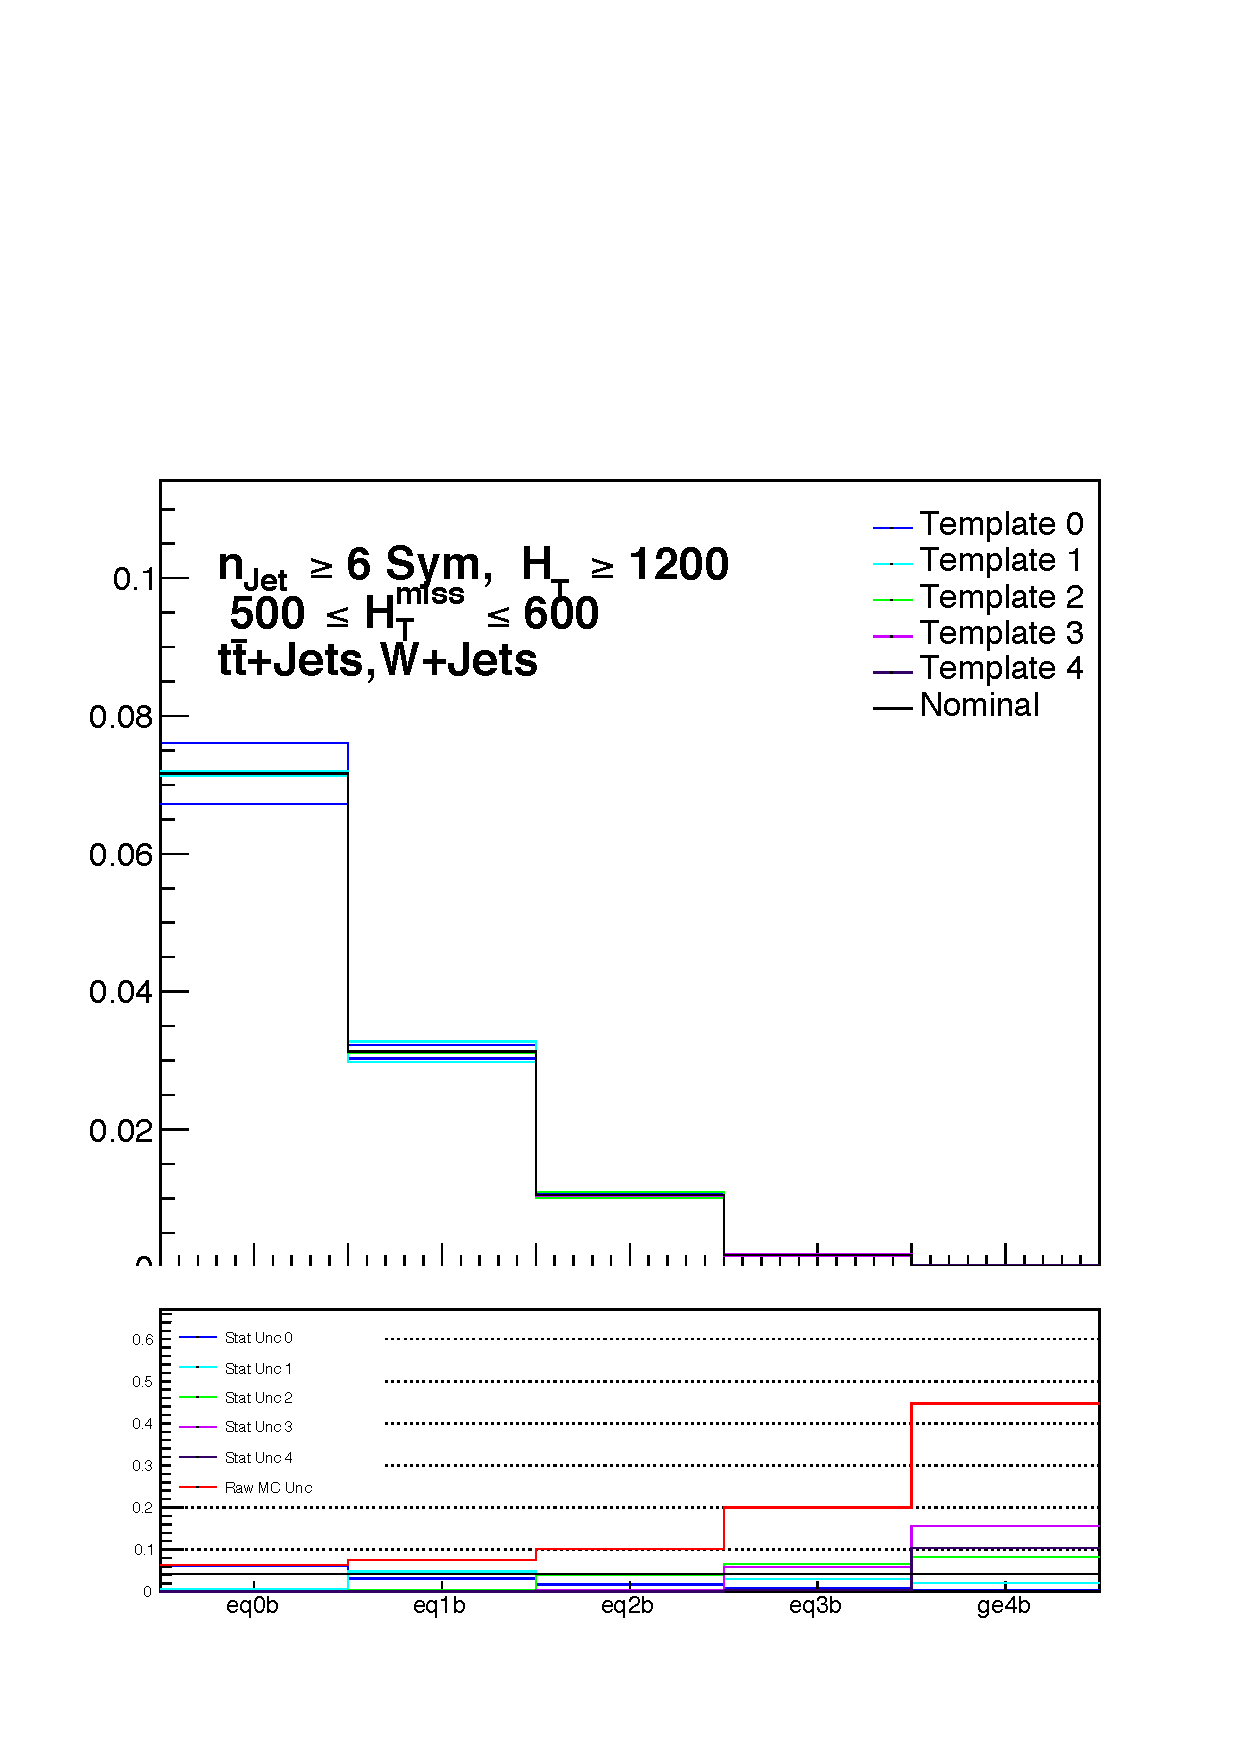
\includegraphics[width=0.45\textwidth]{figures/btagformula/uncertainties/Ttw_ge6j_1200Inc_500600} \\
  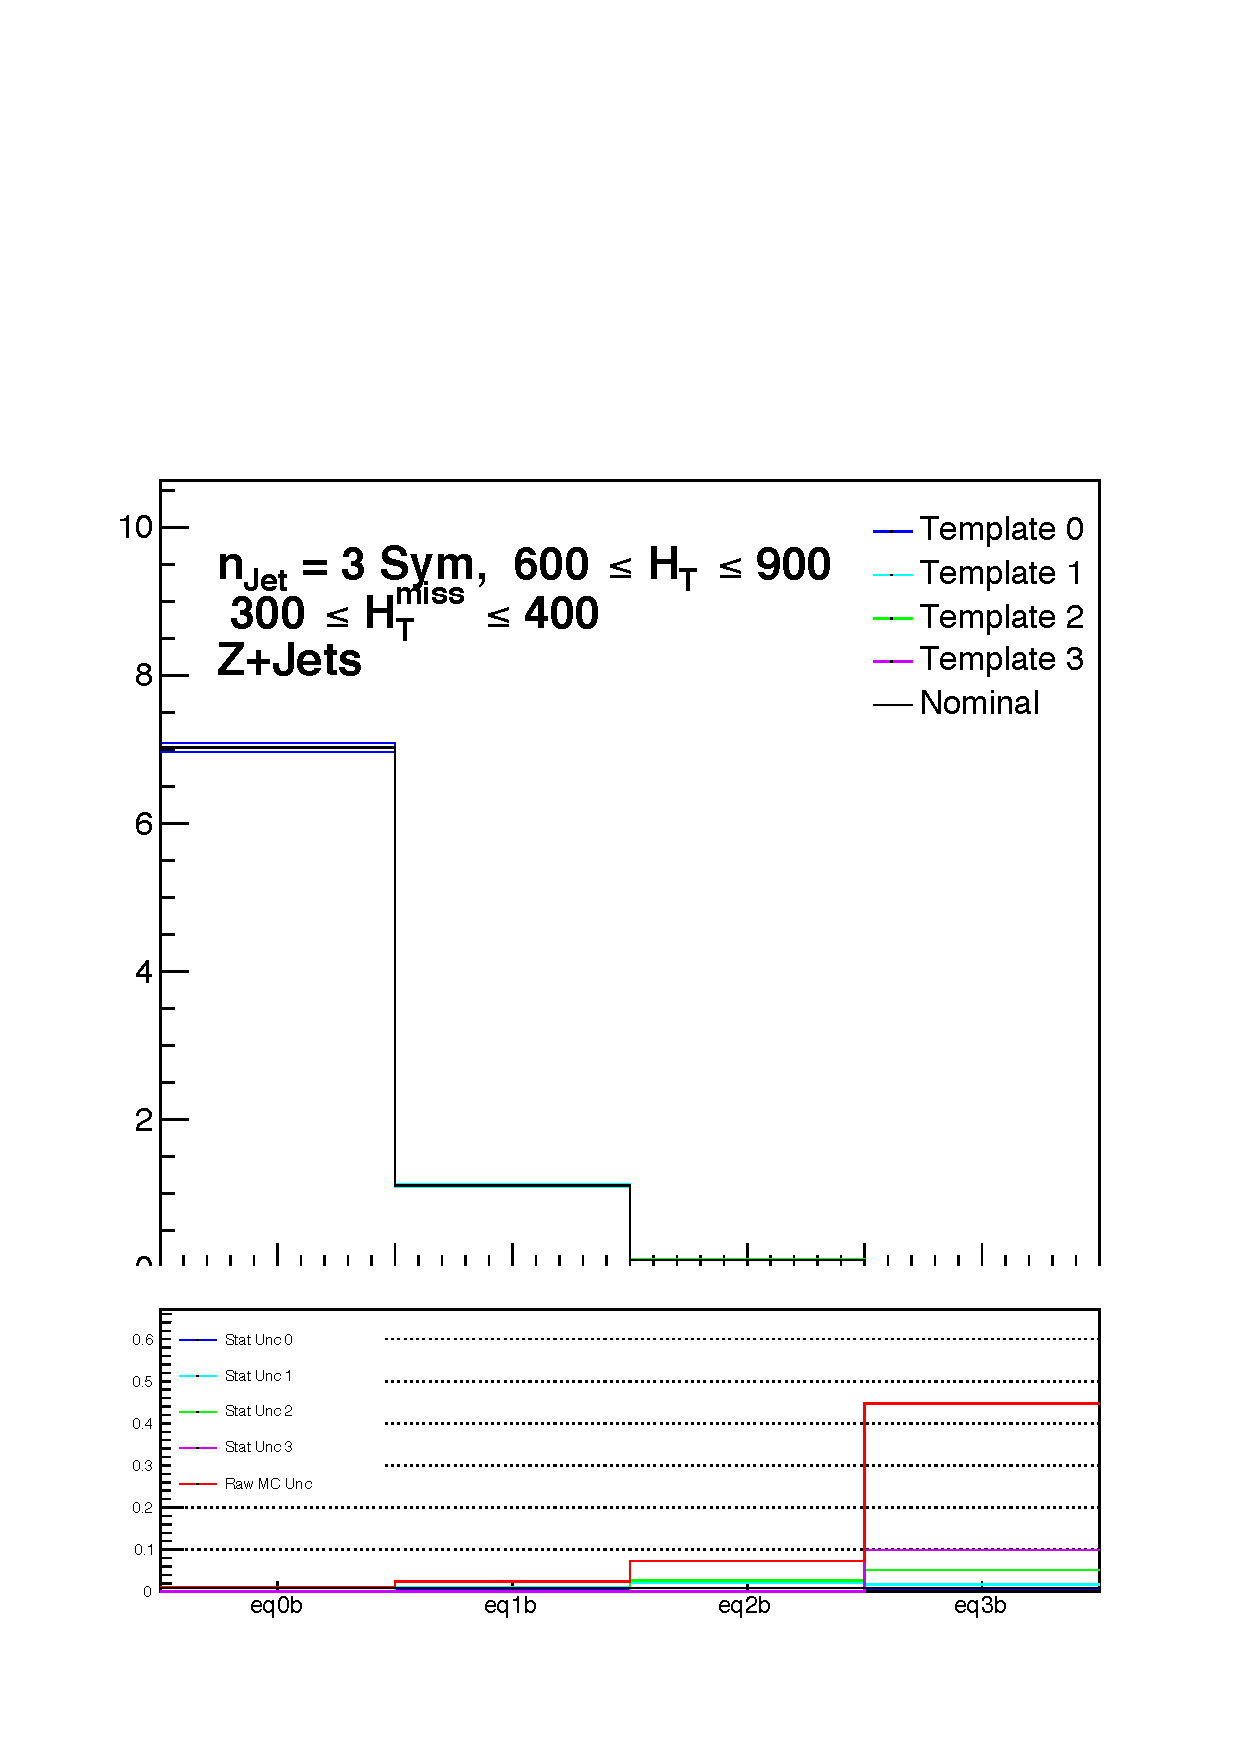
\includegraphics[width=0.45\textwidth]{figures/btagformula/uncertainties/Zinv_eq3j_600900_300400}~
  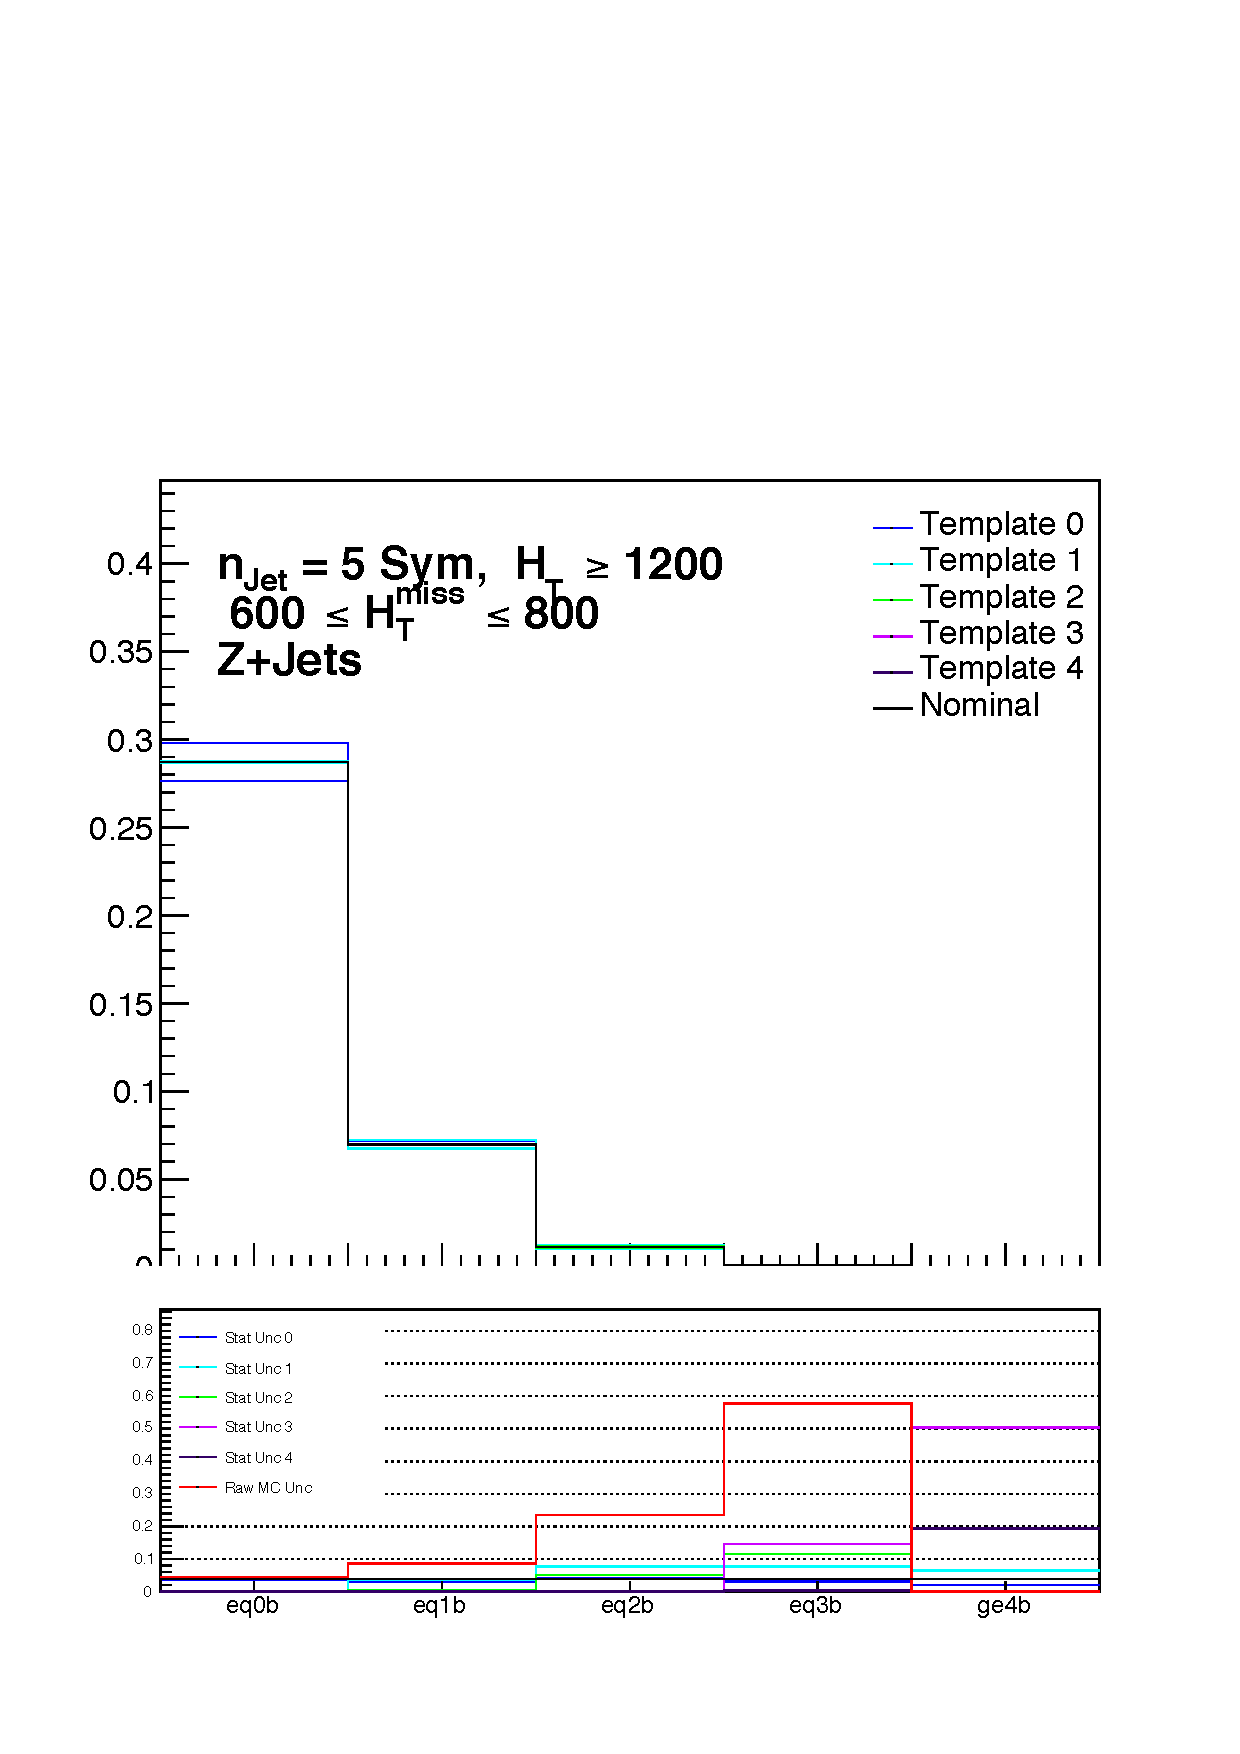
\includegraphics[width=0.45\textwidth]{figures/btagformula/uncertainties/Zinveq5j_1200Inc_600800}
  \caption{\label{fig:formula-uncertainties}
  $n^{\rm tag}$ nominal templates compared to the alternative shapes derived with the toy procedure (``Template0/1/2/3/4'') 
  for the TTJets and WJets processes together (top) and ZToNuNu process (bottom), for some representative (\njet,\scalht,\mht) bins. 
  The bottom pad shows the relative variation with respect to the nominal shape together with the relative statistical uncertainty 
  from the vanilla MC (shown in red).}
\end{figure}
